\documentclass[12pt,a4paper,oneside]{report}

\usepackage[left=3cm,right=2cm,top=2cm,bottom=2.5cm]{geometry}
\usepackage[fontsize=13pt]{scrextend}
\usepackage{fontspec}
\usepackage{amsmath,amssymb}
\usepackage{booktabs}
\usepackage{array}
\usepackage{tabularx}
\usepackage{enumitem}
\usepackage{graphicx}
\usepackage{xcolor}
\usepackage{tikz}
\usepackage{hyperref}
\usepackage{float}
\usepackage[section]{placeins}
\usepackage{setspace}
\usepackage[numbers,sort&compress]{natbib}

\usetikzlibrary{arrows.meta,positioning,shapes.geometric,calc}
\setmainfont{Times New Roman}

\setlength{\parskip}{0.6em}
\setlength{\parindent}{0pt}
\renewcommand{\arraystretch}{1.15}
\renewcommand{\chaptername}{Chương}
\renewcommand{\contentsname}{Mục lục}
\renewcommand{\listfigurename}{Danh mục hình}
\renewcommand{\listtablename}{Danh mục bảng}
\renewcommand{\bibname}{Tài liệu tham khảo}
\renewcommand{\figurename}{Hình}
\renewcommand{\tablename}{Bảng}
\urlstyle{same}
\onehalfspacing

\newcommand{\thesistitlevi}{Nghiên cứu và xây dựng pipeline tái tạo hình học UAV từ ảnh bằng tinh chỉnh chọn lọc theo mức rủi ro}
\newcommand{\studentname}{[Họ và tên sinh viên]}
\newcommand{\studentemail}{[email sinh viên]}
\newcommand{\majorname}{Khoa học máy tính}
\newcommand{\specialization}{Trí tuệ nhân tạo và Thị giác máy tính}
\newcommand{\advisorname}{[Họ tên giảng viên hướng dẫn]}
\newcommand{\departmentname}{[Bộ môn / Bộ phận chuyên môn]}
\newcommand{\schoolname}{Trường Công nghệ Thông tin và Truyền thông}

\hypersetup{
  hidelinks
}

\begin{document}

\begin{titlepage}
\begin{center}
{\large ĐẠI HỌC BÁCH KHOA HÀ NỘI\par}
\vspace{0.3cm}
{\large \schoolname\par}
\vspace{0.8cm}

\includegraphics[width=0.14\textwidth]{figures/web/hust_logo.png}\par
\vspace{1.0cm}
{\Large \textbf{ĐỒ ÁN TỐT NGHIỆP}\par}
\vspace{1.2cm}
{\LARGE \textbf{\thesistitlevi}\par}
\vspace{1.5cm}
\begin{tabular}{rl}
\textbf{Sinh viên:} & \studentname \\
\textbf{Email:} & \studentemail \\
\textbf{Ngành:} & \majorname \\
\textbf{Chuyên ngành:} & \specialization \\
\textbf{Giảng viên hướng dẫn:} & \advisorname \\
\textbf{Bộ môn:} & \departmentname \\
\end{tabular}
\vfill
{\large Hà Nội, tháng 05 năm 2026\par}
\end{center}
\end{titlepage}

\pagenumbering{roman}

\chapter*{Tóm tắt}
\addcontentsline{toc}{chapter}{Tóm tắt}

Đồ án này nghiên cứu bài toán tái tạo hình học từ ảnh UAV trong bối cảnh chi phí tính toán là một ràng buộc quan trọng. Thay vì refine toàn bộ chuỗi ảnh bằng một mô hình mạnh và đắt đỏ, đề tài đề xuất một pipeline \textit{risk-guided hybrid refinement}: trước hết chạy DUSt3R để có lớp hình học thô trên toàn bộ scene, sau đó chấm điểm rủi ro tái tạo cho từng frame dựa trên các thành phần về overlap, texture, depth prior và vị trí nhìn, cuối cùng chỉ refine các frame có rủi ro cao bằng MASt3R. Hệ thống được hiện thực hóa thành một repo độc lập có benchmark, script chạy, chuẩn bị dữ liệu và trực quan hóa. Thực nghiệm được tiến hành trên hai dataset thật là Dronescapes và ODMData. Kết quả cho thấy phương pháp đề xuất cải thiện nhẹ nhưng ổn định so với coarse baseline DUSt3R trên Dronescapes, đồng thời giữ được chất lượng cạnh tranh trong khi chỉ refine một phần nhỏ số frame. Tuy nhiên, phương pháp hiện tại chưa vượt MASt3R full-pass về độ chính xác tuyệt đối. Đóng góp chính của đồ án là xây dựng một pipeline hoàn chỉnh, có thể chạy được trên dữ liệu UAV thật, và chỉ ra rằng selective refinement theo mức rủi ro là một hướng có tiềm năng tốt cho bài toán tái tạo UAV có ràng buộc ngân sách tính toán.

\tableofcontents
\addcontentsline{toc}{chapter}{Danh mục hình}
\listoffigures
\addcontentsline{toc}{chapter}{Danh mục bảng}
\listoftables
\clearpage
\pagenumbering{arabic}

\chapter{Mở đầu}

\section{Lý do chọn đề tài}

Tái tạo không gian 3D từ ảnh UAV là một bài toán trung tâm trong photogrammetry, bản đồ số, khảo sát hiện trạng, giám sát công trình và robot thị giác \citep{Colomina2014Unmanned}. Sự phát triển của cảm biến giá rẻ, UAV dân dụng và hạ tầng tính toán đã khiến việc thu nhận dữ liệu ảnh từ trên không trở nên phổ biến hơn rất nhiều. Tuy nhiên, khi khối lượng ảnh tăng lên, bài toán không còn chỉ là dựng được mô hình 3D, mà là dựng được mô hình đó với mức chi phí tính toán có thể chấp nhận được.

Các pipeline cổ điển như SfM kết hợp MVS có thể cho chất lượng hình học cao, nhưng chi phí chạy và công đoạn cài đặt tương đối lớn \citep{Schonberger2016SfM,Jiang2020Efficient,Liao2024High}. Ở chiều ngược lại, các mô hình pointmap gần đây như DUSt3R và MASt3R giúp đơn giản hóa đáng kể việc suy luận hình học trực tiếp từ ảnh \citep{Wang2024DUSt3R,Leroy2024MASt3R}. Dù vậy, việc chạy full-pass các mô hình nặng trên toàn bộ chuỗi ảnh vẫn đặt ra áp lực lớn về thời gian và tài nguyên.

\begin{figure}[H]
\centering
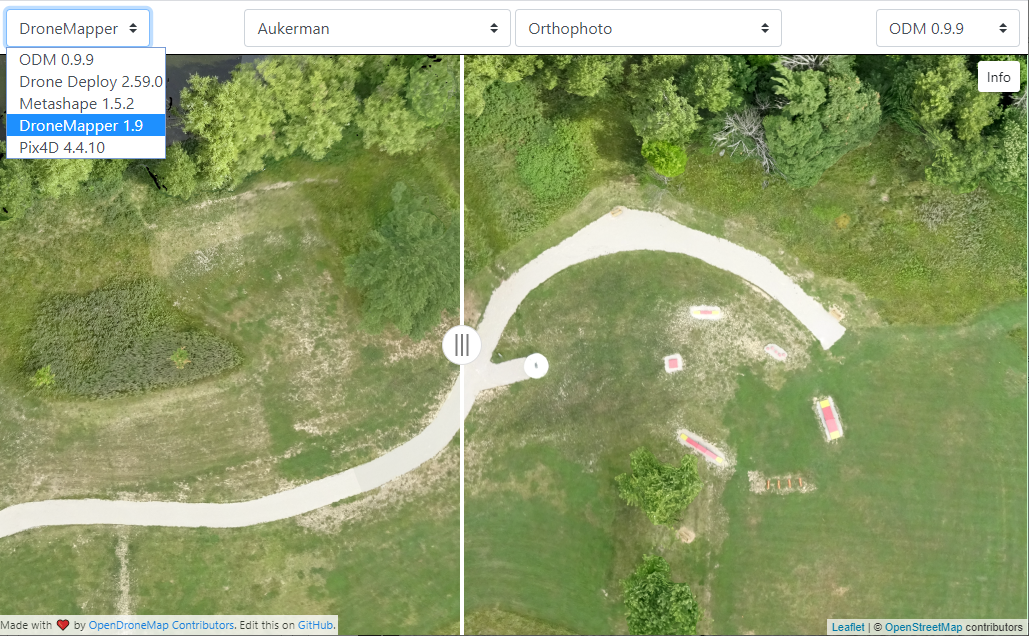
\includegraphics[width=0.88\textwidth]{figures/web/odm_uav_arena.png}
\caption{Một ví dụ benchmark UAV mapping trong hệ sinh thái OpenDroneMap. Hình này cho thấy rõ bối cảnh ứng dụng thực tế của bài toán: từ cùng một block ảnh UAV, hệ thống cần tạo ra các đầu ra hình học hoặc bản đồ có chất lượng tốt, đồng thời chi phí xử lý vẫn phải nằm trong mức chấp nhận được. Nguồn: OpenDroneMap UAV Mapping Arena.}
\label{fig:motivation-uav-budget}
\end{figure}

Từ quan sát này, đề tài lựa chọn một câu hỏi thực dụng hơn: có nhất thiết phải refine toàn bộ frame hay không? Nếu có thể phát hiện những frame có rủi ro tái tạo cao và chỉ dồn ngân sách refine vào đó, pipeline có thể đạt được một điểm cân bằng tốt hơn giữa chất lượng và chi phí.

\section{Mục tiêu của đồ án}

Đồ án hướng đến bốn mục tiêu:
\begin{enumerate}[leftmargin=1.5em]
  \item khảo sát có hệ thống các hướng tiếp cận chính trong 3D reconstruction, đặc biệt là các nhánh liên quan trực tiếp tới ảnh UAV;
  \item đề xuất một chiến lược \textit{risk-guided selective refinement} cho tái tạo hình học từ ảnh UAV;
  \item xây dựng một pipeline benchmark độc lập, có khả năng chuẩn bị dữ liệu, chạy mô hình, so sánh baseline và xuất báo cáo;
  \item đánh giá thực nghiệm phương pháp trên hai dataset thật là Dronescapes và ODMData.
\end{enumerate}

\section{Phạm vi nghiên cứu}

Đề tài tập trung vào bài toán tái tạo hình học từ ảnh UAV trong thiết lập offline, ưu tiên độ ổn định của pipeline benchmark và trade-off giữa chất lượng với chi phí tính toán. Đồ án không theo đuổi các hướng như text-to-3D, human reconstruction hay dynamic scene reconstruction, và cũng không đặt mục tiêu tối ưu rendering hay novel-view synthesis như các hệ NeRF hoặc Gaussian Splatting thuần túy.

\section{Đóng góp của đồ án}

Các đóng góp chính gồm:
\begin{enumerate}[leftmargin=1.5em]
  \item hệ thống hóa bối cảnh nghiên cứu về 3D reconstruction và xác định vị trí của bài toán UAV reconstruction trong hệ sinh thái đó;
  \item đề xuất và hiện thực hóa một pipeline \textit{risk-guided hybrid refinement} kết hợp DUSt3R và MASt3R;
  \item xây dựng repo GEO như một framework benchmark độc lập cho UAV reconstruction;
  \item cung cấp kết quả thực nghiệm định lượng và định tính trên hai dataset thật, kèm phân tích điểm mạnh, điểm yếu và giới hạn của phương pháp.
\end{enumerate}

\section{Bố cục báo cáo}

Báo cáo được tổ chức như sau. Chương 2 trình bày tổng quan về 3D reconstruction và khảo sát các hướng tiếp cận chính. Chương 3 tóm tắt cơ sở lý thuyết cần cho đề tài. Chương 4 mô tả giải pháp đề xuất. Chương 5 trình bày thiết kế và cài đặt hệ thống GEO. Chương 6 trình bày thực nghiệm và đánh giá. Chương 7 kết luận và nêu hướng phát triển tiếp theo.

\chapter{Tổng quan về 3D Reconstruction và các hướng nghiên cứu liên quan}

\section{Khái quát bài toán 3D reconstruction}

3D reconstruction là bài toán khôi phục một biểu diễn hình học của đối tượng hoặc môi trường từ dữ liệu quan sát. Tùy theo đầu vào, đầu ra và mục tiêu cuối cùng, một hệ reconstruction có thể sinh ra point cloud, depth map, mesh, volumetric representation hoặc các biểu diễn liên tục như neural field. Trong bối cảnh UAV, đầu vào thường là tập ảnh RGB đa góc nhìn; đầu ra mong muốn có thể là depth map, point cloud, orthomosaic, DSM hoặc một mô hình 3D có thể phục vụ khảo sát và phân tích địa không gian.

\section{Phân loại các hướng tiếp cận chính}

\begin{table}[t]
\centering
\small
\begin{tabularx}{\textwidth}{>{\raggedright\arraybackslash}p{3.5cm} >{\raggedright\arraybackslash}X >{\raggedright\arraybackslash}p{3.4cm}}
\toprule
\textbf{Nhánh nghiên cứu} & \textbf{Ý tưởng chính} & \textbf{Mức độ liên quan tới đề tài} \\
\midrule
SfM/MVS cổ điển & Khôi phục pose camera và cấu trúc thưa, sau đó dựng depth hoặc point cloud dày & Rất cao \\
Single-view 3D reconstruction & Suy ra 3D từ một ảnh đơn nhờ prior học được & Trung bình \\
RGB-D/LiDAR fusion & Kết hợp ảnh với cảm biến độ sâu để tăng độ chính xác hình học & Trung bình \\
NeRF và neural radiance fields & Học biểu diễn liên tục cho novel-view synthesis và scene rendering & Trung bình \\
3D Gaussian Splatting & Dùng Gaussian 3D explicit cho scene representation và rendering nhanh & Trung bình \\
Feed-forward multi-view reconstruction & Suy luận geometry trực tiếp từ nhiều ảnh bằng mô hình học sâu & Rất cao \\
SLAM kết hợp reconstruction & Vừa định vị vừa dựng bản đồ trong thời gian thực hoặc gần thời gian thực & Cao \\
\bottomrule
\end{tabularx}
\caption{Các hướng nghiên cứu lớn của 3D reconstruction và mức độ liên quan tới đề tài.}
\label{tab:survey-directions}
\end{table}

Bảng \ref{tab:survey-directions} cho thấy đề tài này đứng tại giao của ba hướng: reconstruction từ ảnh đa góc nhìn, geometric learning theo kiểu feed-forward, và selective processing dưới ràng buộc ngân sách tính toán.

\begin{figure}[H]
\centering
\resizebox{0.92\textwidth}{!}{%
\begin{tikzpicture}[
  node distance=0.8cm and 0.9cm,
  every node/.style={font=\scriptsize},
  group/.style={rounded corners, draw=black!65, very thick, align=center, minimum height=1.2cm, text width=3.1cm, fill=blue!8},
  core/.style={rounded corners, draw=red!70!black, very thick, align=center, minimum height=1.0cm, text width=3.5cm, fill=red!10},
  thesis/.style={rounded corners, draw=green!50!black, very thick, align=center, minimum height=1.1cm, text width=3.7cm, fill=green!12},
  arrow/.style={-{Latex[length=3mm]}, thick}
]
\node[core] (main) {3D reconstruction\\từ ảnh và cảm biến};
\node[group, below left=1.5cm and 3.7cm of main] (classical) {Hình học cổ điển\\SfM/MVS, RGB-D, LiDAR};
\node[group, below=1.5cm of main] (scene) {Biểu diễn scene\\NeRF, 3DGS};
\node[group, below right=1.5cm and 3.7cm of main] (learned) {Hình học học sâu\\single-view, feed-forward, SLAM};
\node[thesis, below=2.0cm of scene] (geo) {Đề tài GEO\\UAV multi-view reconstruction\\+ risk-guided selective refinement};

\draw[arrow] (main) -- (classical);
\draw[arrow] (main) -- (scene);
\draw[arrow] (main) -- (learned);
\draw[arrow, green!50!black, very thick] (learned) -- (geo);
\draw[arrow, dashed, green!50!black] (classical.south) to[out=-65,in=170] (geo.west);
\end{tikzpicture}
}
\caption{Bản đồ khái niệm rút gọn của các họ phương pháp chính trong 3D reconstruction. Đề tài GEO nằm gần nhánh hình học học sâu, nhưng vẫn thừa hưởng tư duy đánh giá và benchmark từ nhánh hình học cổ điển.}
\label{fig:reconstruction-taxonomy}
\end{figure}

\section{SfM/MVS và photogrammetry cổ điển}

Đây là nhánh kinh điển và vẫn rất quan trọng đối với ảnh UAV. Trong một pipeline điển hình, SfM dùng feature matching, geometric verification và bundle adjustment để khôi phục pose camera cùng point cloud thưa \citep{Schonberger2016SfM,Jiang2017Efficient,Jiang2020Efficient}. Sau đó, MVS tạo ra point cloud dày hoặc depth map bằng cách khai thác thông tin đa góc nhìn \citep{Liu2023Deep,Liao2024High}. Các công trình trong nhánh này rất mạnh về hình học, nhưng thường đánh đổi bằng chi phí tính toán và độ phức tạp cài đặt.

\begin{figure}[H]
\centering
\begin{tikzpicture}[
  node distance=0.7cm and 0.55cm,
  stage/.style={rounded corners, draw=black!65, very thick, align=center, minimum height=1cm, text width=2.45cm, fill=blue!8},
  outbox/.style={rounded corners, draw=green!45!black, very thick, align=center, minimum height=1cm, text width=2.5cm, fill=green!12},
  arrow/.style={-{Latex[length=3mm]}, thick}
]
\node[stage] (img) {Ảnh UAV\\đa góc nhìn};
\node[stage, right=of img] (feat) {Trích xuất\\đặc trưng};
\node[stage, right=of feat] (match) {Matching +\\kiểm định hình học};
\node[stage, right=of match] (sfm) {SfM + bundle\\adjustment};
\node[outbox, below=1.1cm of sfm] (sparse) {Sparse point cloud\\và pose camera};
\node[stage, left=of sparse] (mvs) {Multi-view\\stereo};
\node[outbox, left=of mvs] (dense) {Dense point cloud /\\depth / DSM};

\draw[arrow] (img) -- (feat);
\draw[arrow] (feat) -- (match);
\draw[arrow] (match) -- (sfm);
\draw[arrow] (sfm) -- (sparse);
\draw[arrow] (sparse) -- (mvs);
\draw[arrow] (mvs) -- (dense);
\end{tikzpicture}
\caption{Pipeline khái quát của nhánh SfM/MVS cổ điển. Ưu điểm của hướng này là hình học chặt, nhưng đổi lại là chuỗi xử lý dài và chi phí tính toán cao hơn.}
\label{fig:sfm-mvs-pipeline}
\end{figure}

\section{Neural reconstruction và feed-forward geometry}

Sự xuất hiện của DUSt3R và MASt3R đã mở ra một hướng mới: mô hình học sâu suy luận geometry trực tiếp từ tập ảnh mà không cần giữ nguyên toàn bộ cấu trúc photogrammetry cổ điển \citep{Wang2024DUSt3R,Leroy2024MASt3R}. DUSt3R dự báo pointmap hoặc depth-like structure trực tiếp, trong khi MASt3R cải thiện mạnh matching và độ nhất quán hình học. Trên các aerial blocks, các mô hình này cho thấy tiềm năng tốt trong những vùng khó và block thưa \citep{Wu2025AerialBlocks}.

Tuy nhiên, nhược điểm vẫn còn là chi phí full-pass trên toàn bộ tập ảnh. Đây chính là điểm nối tự nhiên sang bài toán selective refinement.

\begin{figure}[H]
\centering
\begin{minipage}[t]{0.47\textwidth}
  \centering
  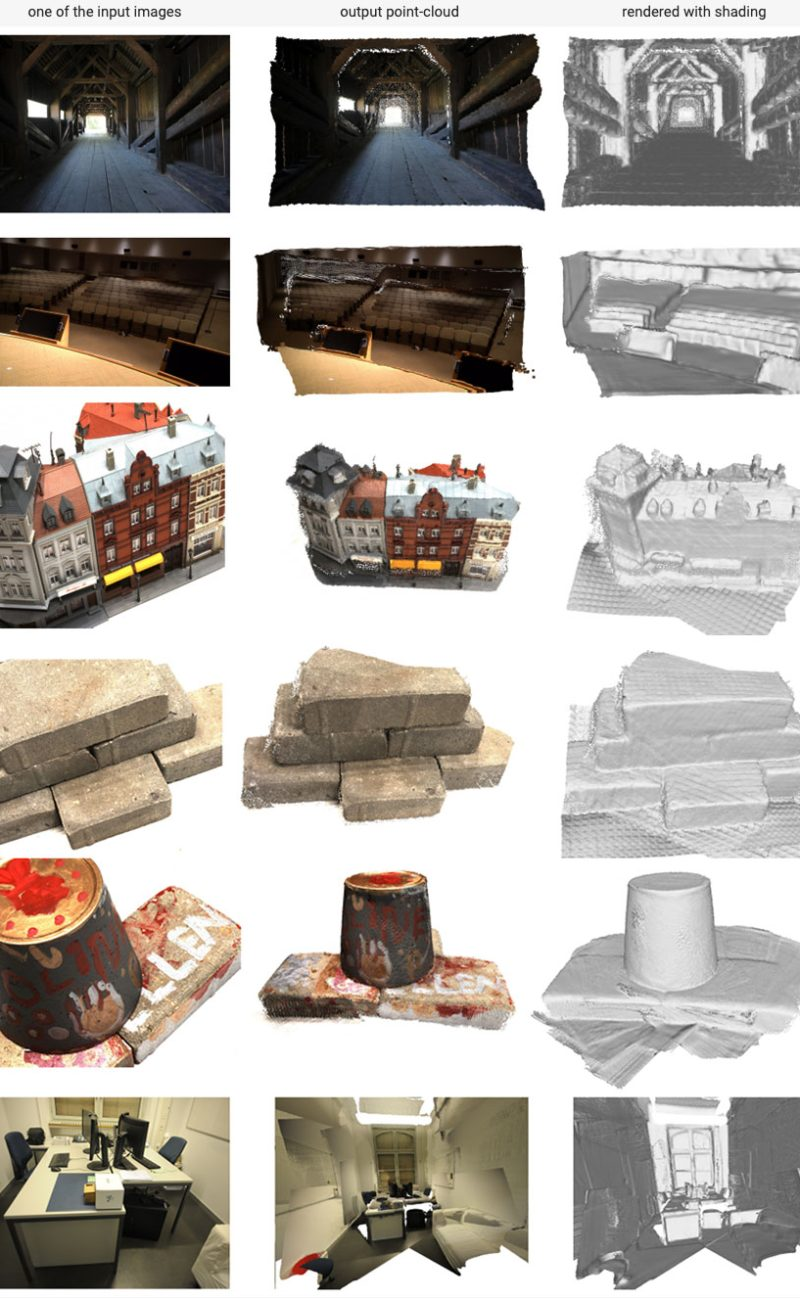
\includegraphics[width=\linewidth]{figures/web/dust3r_result.jpg}

  \scriptsize (a) Minh họa đầu vào--đầu ra của DUSt3R: từ một cặp ảnh tới point cloud và phối cảnh có tô bóng.
\end{minipage}
\hfill
\begin{minipage}[t]{0.47\textwidth}
  \centering
  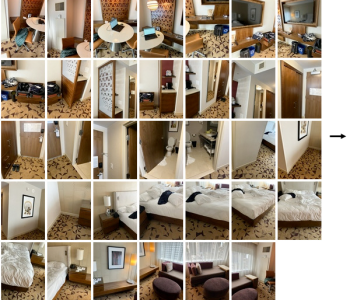
\includegraphics[width=\linewidth]{figures/web/mast3r_room.png}

  \scriptsize (b) Bối cảnh multi-view dày và chồng lấp mạnh, nơi các mô hình kiểu MASt3R phát huy ưu thế về matching và nhất quán hình học.
\end{minipage}

\vspace{0.8em}

\begin{minipage}{0.70\textwidth}
  \centering
  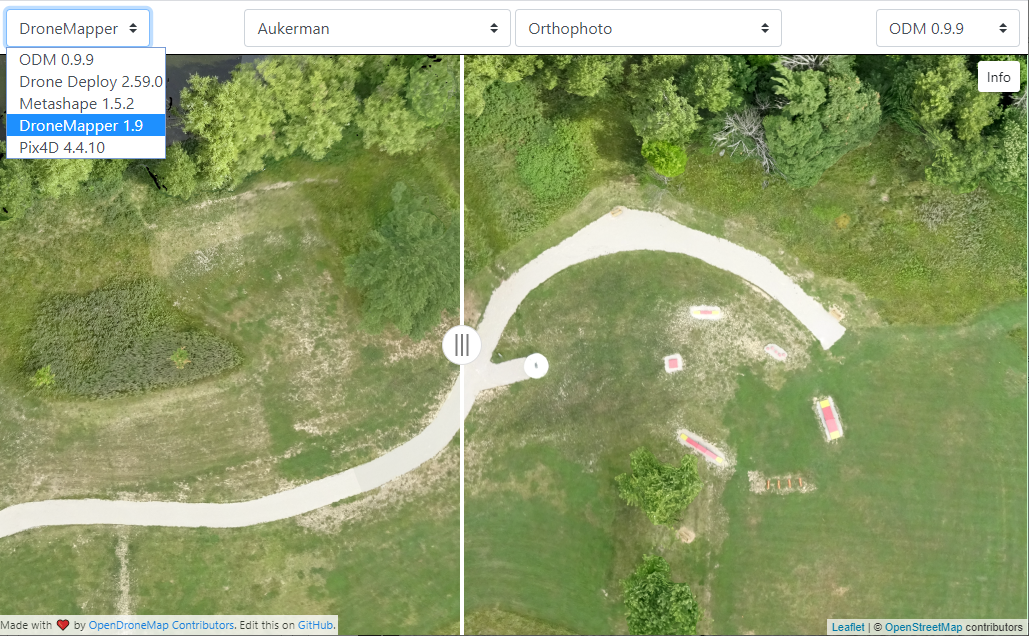
\includegraphics[width=\linewidth]{figures/web/odm_uav_arena.png}

  \scriptsize (c) Một ví dụ benchmark photogrammetry UAV trong hệ sinh thái OpenDroneMap, cho thấy nhu cầu so sánh tái tạo trên các block bay thật.
\end{minipage}
\caption{Cụm hình ngữ cảnh cho ba lớp vấn đề mà đồ án quan tâm: geometry từ mô hình feed-forward, bài toán matching đa góc nhìn, và benchmark trên dữ liệu UAV thật. Các hình được lấy từ tư liệu kỹ thuật chính thức của DUSt3R, MASt3R và OpenDroneMap.}
\label{fig:contextual-banners}
\end{figure}

\section{NeRF, Gaussian Splatting và scene representation}

NeRF và các biến thể neural radiance field hướng tới việc học một biểu diễn liên tục của scene để render novel views chất lượng cao \citep{Wei2024LiDeNeRF}. Sau đó, 3D Gaussian Splatting đưa ra một biểu diễn explicit hơn, giúp render nhanh hơn và thuận lợi cho các ứng dụng visual scene representation \citep{Yao2026ARSGaussian}. Dù rất quan trọng trong bức tranh tổng thể của 3D reconstruction, các phương pháp này không phải trục chính của đồ án hiện tại vì chúng thiên về rendering và scene representation hơn là depth-centric geometry benchmark dưới ngân sách giới hạn.

\begin{figure}[H]
\centering
\begin{minipage}[t]{0.47\textwidth}
\centering
\resizebox{0.92\linewidth}{!}{%
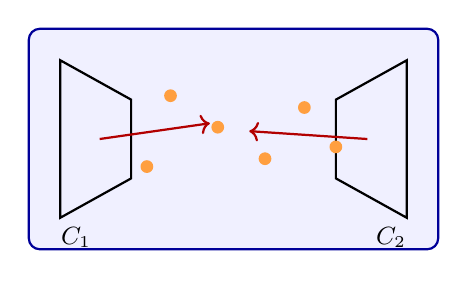
\begin{tikzpicture}[every node/.style={font=\scriptsize}]
\draw[rounded corners, fill=blue!6, draw=blue!60!black, thick] (-2.6,-1.4) rectangle (2.6,1.4);
\draw[thick] (-2.2,-1.0) -- (-1.3,-0.5) -- (-1.3,0.5) -- (-2.2,1.0) -- cycle;
\node at (-2.0,-1.25) {$C_1$};
\draw[thick] (2.2,-1.0) -- (1.3,-0.5) -- (1.3,0.5) -- (2.2,1.0) -- cycle;
\node at (2.0,-1.25) {$C_2$};
\draw[red!70!black, thick, ->] (-1.7,0) -- (-0.3,0.2);
\draw[red!70!black, thick, ->] (1.7,0) -- (0.2,0.1);
\foreach \x/\y in {-0.2/0.15,0.4/-0.25,0.9/0.4,1.3/-0.1,-0.8/0.55,-1.1/-0.35}{
  \fill[orange!75] (\x,\y) circle (2.3pt);
}
\end{tikzpicture}
}

{\scriptsize (a) NeRF: trường liên tục, lấy mẫu theo tia và tích phân thể tích.}
\end{minipage}
\hfill
\begin{minipage}[t]{0.47\textwidth}
\centering
\resizebox{0.92\linewidth}{!}{%
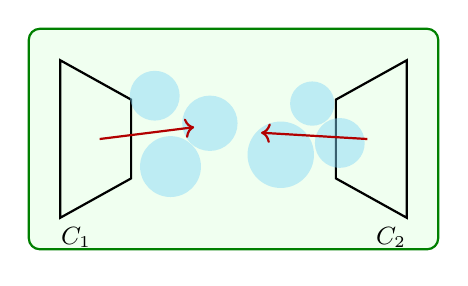
\begin{tikzpicture}[every node/.style={font=\scriptsize}]
\draw[rounded corners, fill=green!6, draw=green!50!black, thick] (-2.6,-1.4) rectangle (2.6,1.4);
\draw[thick] (-2.2,-1.0) -- (-1.3,-0.5) -- (-1.3,0.5) -- (-2.2,1.0) -- cycle;
\node at (-2.0,-1.25) {$C_1$};
\draw[thick] (2.2,-1.0) -- (1.3,-0.5) -- (1.3,0.5) -- (2.2,1.0) -- cycle;
\node at (2.0,-1.25) {$C_2$};
\foreach \x/\y/\r in {-0.3/0.2/10,0.6/-0.2/12,1.0/0.45/8,-1.0/0.55/9,-0.8/-0.35/11,1.35/-0.05/9}{
  \fill[cyan!50, opacity=0.45] (\x,\y) circle (\r pt);
}
\draw[red!70!black, thick, ->] (-1.7,0) -- (-0.5,0.15);
\draw[red!70!black, thick, ->] (1.7,0) -- (0.35,0.08);
\end{tikzpicture}
}

{\scriptsize (b) Gaussian Splatting: dùng các primitive Gaussian explicit để render nhanh hơn.}
\end{minipage}
\caption{Minh họa khái niệm cho hai họ phương pháp scene representation. NeRF biểu diễn scene dưới dạng trường liên tục cần tích phân theo tia nhìn, trong khi Gaussian Splatting dùng các primitive explicit giúp render nhanh hơn.}
\label{fig:nerf-vs-gs}
\end{figure}

\section{Uncertainty, confidence và selective processing}

Trong rất nhiều bài toán dense geometry, confidence và uncertainty đóng vai trò then chốt để kiểm soát chất lượng tái tạo. Ý tưởng chung là không phải mọi quan sát đều đáng tin cậy như nhau; do đó, hệ thống cần có cơ chế đánh giá mức rủi ro hoặc độ chắc chắn để quyết định nên cập nhật mô hình ở đâu và mức nào. Đề tài này tiếp nối tinh thần đó, nhưng đưa nó về mức frame-level selection trong một pipeline UAV reconstruction offline.

\section{Khoảng trống nghiên cứu mà đề tài lựa chọn}

Từ các nhánh trên, có thể rút ra ba nhận xét:
\begin{enumerate}[leftmargin=1.5em]
  \item pipeline cổ điển mạnh về hình học nhưng nặng và khó co giãn theo ngân sách tính toán;
  \item pipeline học sâu mới giúp suy luận geometry dễ hơn, nhưng full-pass trên mọi frame vẫn tốn kém;
  \item số lượng công trình tập trung trực tiếp vào \textit{frame-level refinement budget allocation} trong bài toán UAV reconstruction hiện còn ít.
\end{enumerate}

Đề tài vì thế chọn khoảng trống nghiên cứu sau: \textbf{phân bổ chọn lọc ngân sách refine trong tái tạo hình học UAV bằng một thước đo rủi ro frame-level}.

\chapter{Cơ sở lý thuyết cho bài toán tái tạo UAV từ ảnh}

\section{Hình học camera và phép chiếu phối cảnh}

Trong hệ camera lỗ kim, một điểm 3D $\mathbf{X}$ trong không gian được chiếu lên ảnh thông qua ma trận nội tại $K$ và ngoại tại $[R|t]$. Ở dạng thuần nhất:
\[
\mathbf{x} \sim K [R|t] \mathbf{X}.
\]
Trong các pipeline multi-view, việc ước lượng chính xác pose camera và mối quan hệ hình học giữa các ảnh là điều kiện tiên quyết để có thể khôi phục geometry ổn định.

\begin{figure}[H]
\centering
\resizebox{0.78\textwidth}{!}{%
\begin{tikzpicture}[
  cam/.style={draw=black!70, fill=gray!12, thick},
  plane/.style={draw=blue!60, fill=blue!8, thick},
  ray/.style={-{Latex[length=2.5mm]}, red!70!black, thick},
  guide/.style={dashed, gray!70},
  every node/.style={font=\small}
]
% camera 1
\draw[cam] (-4.8,0) -- (-4.1,0.45) -- (-4.1,-0.45) -- cycle;
\draw[plane] (-3.25,-0.95) rectangle (-3.0,0.95);
\node at (-4.55,-0.8) {$C_1$};
\node[blue!60!black] at (-3.12,1.2) {mặt phẳng ảnh 1};
% camera 2
\draw[cam] (4.8,0) -- (4.1,0.45) -- (4.1,-0.45) -- cycle;
\draw[plane] (3.0,-0.95) rectangle (3.25,0.95);
\node at (4.55,-0.8) {$C_2$};
\node[blue!60!black] at (3.12,1.2) {mặt phẳng ảnh 2};
% world point
\filldraw[red!80!black] (0,1.1) circle (2.2pt);
\node[above] at (0,1.1) {điểm 3D $\mathbf{X}$};
% rays
\draw[ray] (-4.35,0) -- (0,1.1);
\draw[ray] (4.35,0) -- (0,1.1);
% image projections
\filldraw[red!80!black] (-3.12,0.3) circle (2pt);
\filldraw[red!80!black] (3.12,0.3) circle (2pt);
\node[left] at (-3.18,0.3) {$\mathbf{x}_1$};
\node[right] at (3.18,0.3) {$\mathbf{x}_2$};
\draw[guide] (0,1.1) -- (-3.12,0.3);
\draw[guide] (0,1.1) -- (3.12,0.3);
\end{tikzpicture}
}
\caption{Minh họa hình học camera đa góc nhìn trong tái tạo 3D từ ảnh UAV. Hai camera quan sát cùng một điểm 3D từ các pose khác nhau; từ các phép chiếu tương ứng, hệ thống có thể suy ra pose, depth và cấu trúc scene.}
\label{fig:multi-view-geometry}
\end{figure}

\section{Depth map, point cloud và pointmap}

Depth map biểu diễn khoảng cách từ camera tới bề mặt scene tại từng pixel. Point cloud là tập các điểm 3D trong hệ tọa độ thế giới hoặc hệ camera. Pointmap trong các mô hình như DUSt3R là một cách dự báo trực tiếp ánh xạ từ pixel sang tọa độ 3D, giúp đơn giản hóa nhiều bước ràng buộc projective cổ điển.

\begin{figure}[H]
\centering
\begin{minipage}[t]{0.31\textwidth}
  \centering
  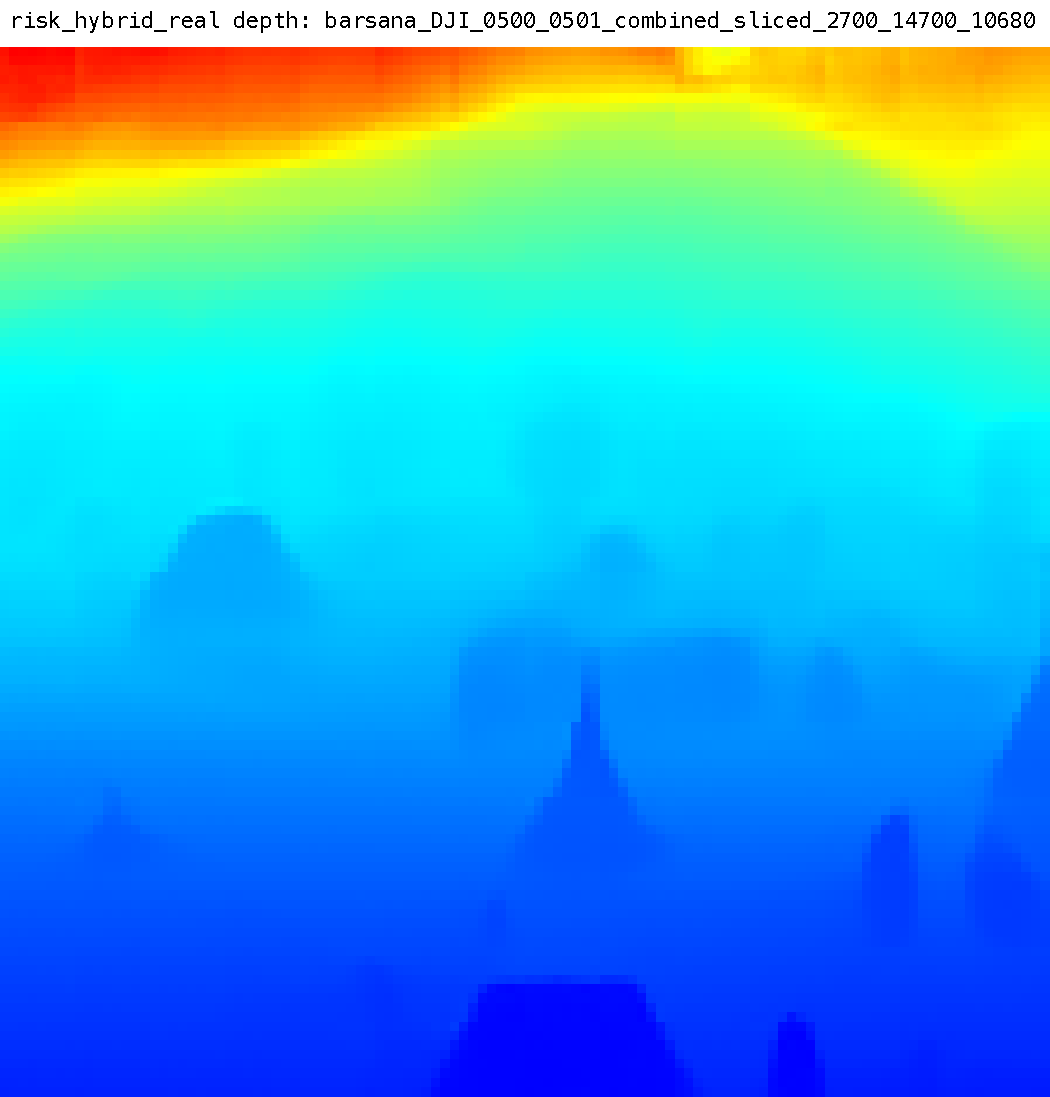
\includegraphics[width=\linewidth]{figures/dronescapes_risk_depth.pdf}

  \scriptsize (a) Depth map
\end{minipage}
\hfill
\begin{minipage}[t]{0.31\textwidth}
  \centering
  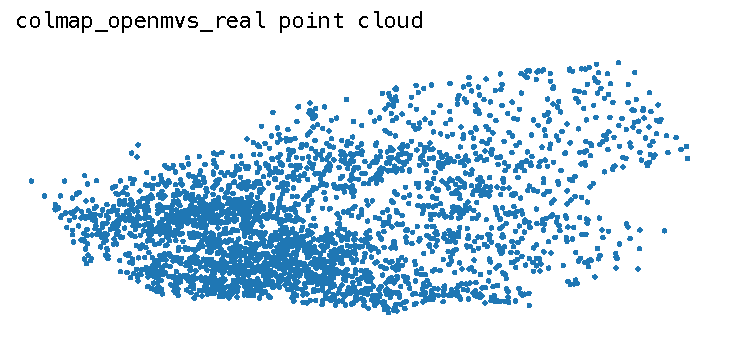
\includegraphics[width=\linewidth]{figures/odmdata_openmvs_pointcloud.pdf}

  \scriptsize (b) Point cloud
\end{minipage}
\hfill
\begin{minipage}[t]{0.31\textwidth}
  \centering
  \begin{tikzpicture}[scale=0.8, every node/.style={font=\scriptsize}]
    \draw[fill=gray!12, draw=black!70] (-1.3,-1.0) rectangle (0.2,1.0);
    \draw[step=0.3, gray!55] (-1.3,-1.0) grid (0.2,1.0);
    \node at (-0.55,1.25) {pixel grid};
    \foreach \x/\y/\tx/\ty in {-1.05/0.65/1.1/1.0,-0.75/0.05/1.45/0.4,-0.45/-0.55/0.95/-0.65,-1.15/-0.2/1.65/-0.1}{
      \fill[red!70!black] (\x,\y) circle (1.8pt);
      \fill[blue!65] (\tx,\ty) circle (2pt);
      \draw[->, thick, orange!80!black] (\x,\y) -- (\tx,\ty);
    }
    \draw[thick] (1.0,-0.9) -- (2.0,-0.5) -- (1.6,0.9);
    \draw[thick] (1.0,-0.9) -- (1.25,-0.15) -- (1.6,0.9);
    \draw[thick] (2.0,-0.5) -- (1.25,-0.15);
    \node at (1.35,1.25) {tọa độ 3D};
    \node[align=center] at (0.4,-1.35) {Pointmap: mỗi pixel\\được ánh xạ sang một điểm 3D};
  \end{tikzpicture}

  \scriptsize (c) Pointmap
\end{minipage}
\caption{Ba kiểu biểu diễn hình học xuất hiện xuyên suốt đồ án. Depth map thuận tiện cho đánh giá theo pixel; point cloud phù hợp quan sát cấu trúc scene; pointmap giúp mô hình học sâu dự báo trực tiếp hình học 3D từ miền ảnh.}
\label{fig:depth-pointcloud-pointmap}
\end{figure}

\section{Các yếu tố làm khó tái tạo UAV}

Với ảnh UAV, các khó khăn chính thường đến từ:
\begin{enumerate}[leftmargin=1.5em]
  \item texture yếu hoặc lặp lại, khiến matching kém ổn định;
  \item overlap không đều giữa các ảnh;
  \item góc nhìn bất lợi, đặc biệt với các cấu trúc hẹp hoặc che khuất;
  \item thay đổi cao độ, ánh sáng, hoặc cảnh quá rộng làm tăng chi phí tính toán.
\end{enumerate}

Những yếu tố này chính là nền tảng để xây dựng một thước đo \textit{reconstruction risk}.

\begin{figure}[H]
\centering
\begin{minipage}[t]{0.47\textwidth}
\centering
\resizebox{0.95\linewidth}{!}{%
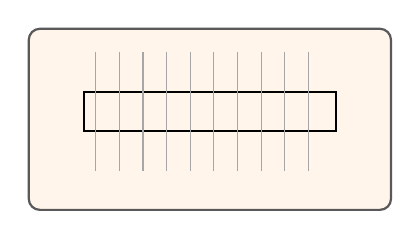
\begin{tikzpicture}[every node/.style={font=\scriptsize}]
\draw[rounded corners, draw=black!65, thick, fill=orange!8] (-2.3,-1.15) rectangle (2.3,1.15);
\draw[thick] (-1.6,-0.15) rectangle (1.6,0.35);
\foreach \x in {-1.45,-1.15,-0.85,-0.55,-0.25,0.05,0.35,0.65,0.95,1.25}{
  \draw[gray!70] (\x,-0.65) -- (\x,0.85);
}
\end{tikzpicture}
}

{\scriptsize \textbf{(a) Texture yếu hoặc lặp lại.} Matching dễ mơ hồ ở mái nhà, đường, đồng cỏ hoặc các mặt phẳng lớn.}
\end{minipage}
\hfill
\begin{minipage}[t]{0.47\textwidth}
\centering
\resizebox{0.95\linewidth}{!}{%
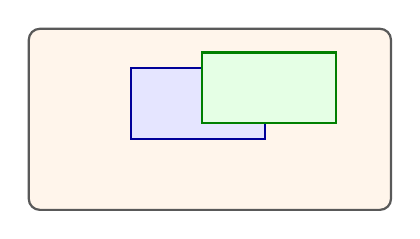
\begin{tikzpicture}[every node/.style={font=\scriptsize}]
\draw[rounded corners, draw=black!65, thick, fill=orange!8] (-2.3,-1.15) rectangle (2.3,1.15);
\draw[fill=blue!10, draw=blue!60!black, thick] (-1.0,-0.25) rectangle (0.7,0.65);
\draw[fill=green!10, draw=green!50!black, thick] (-0.1,-0.05) rectangle (1.6,0.85);
\end{tikzpicture}
}

{\scriptsize \textbf{(b) Overlap không đều.} Các cặp ảnh hỗ trợ hình học không phân bố đồng đều trên toàn block bay.}
\end{minipage}

\vspace{0.7em}

\begin{minipage}[t]{0.47\textwidth}
\centering
\resizebox{0.95\linewidth}{!}{%
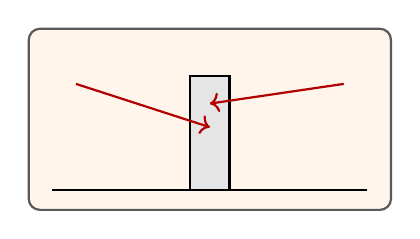
\begin{tikzpicture}[every node/.style={font=\scriptsize}]
\draw[rounded corners, draw=black!65, thick, fill=orange!8] (-2.3,-1.15) rectangle (2.3,1.15);
\draw[thick] (-2.0,-0.9) -- (2.0,-0.9);
\draw[thick, fill=gray!20] (-0.25,-0.9) rectangle (0.25,0.55);
\draw[->, thick, red!70!black] (-1.7,0.45) -- (0.0,-0.1);
\draw[->, thick, red!70!black] (1.7,0.45) -- (0.0,0.2);
\end{tikzpicture}
}

{\scriptsize \textbf{(c) Góc nhìn bất lợi và che khuất.} Vật thể mảnh, góc xiên và vùng bị che làm depth suy giảm ổn định.}
\end{minipage}
\hfill
\begin{minipage}[t]{0.47\textwidth}
\centering
\resizebox{0.95\linewidth}{!}{%
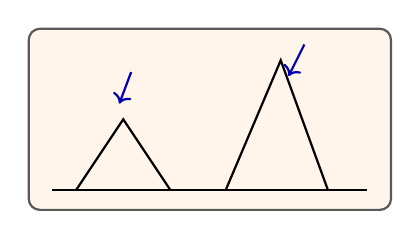
\begin{tikzpicture}[every node/.style={font=\scriptsize}]
\draw[rounded corners, draw=black!65, thick, fill=orange!8] (-2.3,-1.15) rectangle (2.3,1.15);
\draw[thick] (-2.0,-0.9) -- (2.0,-0.9);
\draw[thick] (-1.7,-0.9) -- (-1.1,0.0) -- (-0.5,-0.9);
\draw[thick] (0.2,-0.9) -- (0.9,0.75) -- (1.5,-0.9);
\draw[->, thick, blue!70!black] (-1.0,0.6) -- (-1.15,0.2);
\draw[->, thick, blue!70!black] (1.2,0.95) -- (1.0,0.55);
\end{tikzpicture}
}

{\scriptsize \textbf{(d) Biến thiên cao độ và tỉ lệ.} Đồi dốc hoặc đô thị dày đặc làm thay đổi scale, depth range và phân bố lỗi.}
\end{minipage}
\caption{Bốn tình huống điển hình khiến tái tạo UAV khó ổn định. Đây cũng là các tín hiệu trực giác được chuyển hóa thành những thành phần của risk score trong đồ án.}
\label{fig:uav-difficulty-factors}
\end{figure}

\section{Khái niệm risk score trong đề tài}

Đề tài không học trực tiếp uncertainty bằng một mạng riêng, mà dùng một thước đo heuristic ở mức frame. Mục tiêu của risk score không phải dự báo sai số tuyệt đối, mà trả lời câu hỏi thực dụng hơn: frame nào đáng được refine trước nếu chỉ có một ngân sách hữu hạn?

\begin{figure}[H]
\centering
\begin{tikzpicture}[
  every node/.style={font=\small},
  sel/.style={fill=red!70!black},
  base/.style={fill=blue!55}
]
\draw[->, thick] (0,0) -- (9.2,0) node[right] {frame};
\draw[->, thick] (0,0) -- (0,4.8) node[above] {risk};
\foreach \x/\h/\label in {0.7/1.1/F1,1.7/2.7/F2,2.7/1.8/F3,3.7/4.0/F4,4.7/1.5/F5,5.7/3.6/F6,6.7/0.9/F7,7.7/3.1/F8}{
  \ifdim \h pt>3.0pt
    \fill[sel] (\x,0) rectangle +(0.65,\h);
  \else
    \fill[base] (\x,0) rectangle +(0.65,\h);
  \fi
  \node[below] at (\x+0.325,0) {\label};
}
\draw[dashed, gray!70] (0,3.0) -- (8.7,3.0);
\node[gray!70, anchor=west] at (8.75,3.0) {ngưỡng chọn top-$K$};
\node[align=center] at (4.4,4.35) {\textbf{Các frame rủi ro cao}\\được ưu tiên refine};
\end{tikzpicture}
\caption{Ví dụ trực quan của cơ chế risk-guided selection trong đồ án. Những frame có điểm rủi ro cao hơn được ưu tiên đưa vào nhánh refine, thay vì chạy refinement đồng đều trên toàn bộ chuỗi ảnh.}
\label{fig:risk-selection-theory}
\end{figure}

\chapter{Giải pháp đề xuất: Risk-Guided Hybrid Refinement}

\section{Phát biểu bài toán}

Cho tập ảnh UAV $\mathcal{I}=\{I_i\}_{i=1}^{N}$, mục tiêu là sinh ra một đầu ra hình học đủ tốt trong khi tránh refine toàn bộ frame. Gọi $\mathcal{S}$ là tập frame được chọn để refine, ta muốn tìm một chiến lược sao cho:
\[
\min_{\mathcal{S}} \; \mathcal{L}_{geo}(\hat{\mathcal{D}}(\mathcal{I}, \mathcal{S})) + \lambda \mathcal{C}(\mathcal{S}),
\]
trong đó $\mathcal{L}_{geo}$ đo lỗi hình học sau khi hợp nhất coarse và refine, còn $\mathcal{C}(\mathcal{S})$ đo chi phí suy luận tăng thêm.

\section{Ý tưởng chính}

Thay vì chạy MASt3R trên toàn bộ tập ảnh, đề tài đề xuất:
\begin{enumerate}[leftmargin=1.5em]
  \item chạy DUSt3R toàn cục để có lớp geometry thô;
  \item chấm điểm rủi ro cho từng frame;
  \item chọn top-$K$ frame có rủi ro cao nhất;
  \item refine chúng bằng MASt3R;
  \item hợp nhất coarse prediction và refined prediction thành đầu ra cuối.
\end{enumerate}

\section{Công thức risk score}

Trong implementation hiện tại:
\[
R_i = 0.35 O_i + 0.25 T_i + 0.20 D_i + 0.20 V_i,
\]
trong đó:
\begin{itemize}[leftmargin=1.5em]
  \item $O_i$ là thành phần overlap;
  \item $T_i$ là thành phần texture;
  \item $D_i$ là thành phần depth prior;
  \item $V_i$ là thành phần viewpoint.
\end{itemize}

\textbf{Overlap term.} Thành phần này tăng khi một frame nhận được ít hỗ trợ hình học từ các frame lân cận. Trong code, nó được xấp xỉ từ one-minus-average cosine similarity giữa các ảnh xám lân cận.

\textbf{Texture term.} Thành phần này tăng khi độ lệch chuẩn mức xám thấp, tức vùng ảnh nghèo texture hơn và dễ dẫn đến matching kém ổn định.

\textbf{Depth term.} Thành phần này phản ánh độ phân tán của prior depth nếu có. Trong các run benchmark chính của đề tài, thành phần này thường không phải nguồn phân biệt mạnh nhất, nhưng vẫn được giữ trong formulation để pipeline có thể mở rộng sau này.

\textbf{View term.} Thành phần này phản ánh mức bất lợi của vị trí nhìn trong chuỗi, được xấp xỉ bằng khoảng cách chuẩn hóa tới trung tâm của chuỗi ảnh.

\begin{figure}[H]
\centering
\begin{tikzpicture}[
  block/.style={rounded corners, draw=black!65, thick, align=center, minimum height=1cm, text width=2.7cm, fill=blue!8},
  select/.style={rounded corners, draw=orange!80!black, thick, align=center, minimum height=1cm, text width=2.8cm, fill=orange!15},
  result/.style={rounded corners, draw=green!50!black, thick, align=center, minimum height=1cm, text width=3cm, fill=green!12},
  arrow/.style={-{Latex[length=3mm]}, thick}
]
\node[block] (coarse) {DUSt3R\\coarse pass};
\node[block, right=1.2cm of coarse] (factors) {Overlap\\Texture\\Depth prior\\Viewpoint};
\node[select, right=1.2cm of factors] (risk) {Tính risk score\\cho từng frame};
\node[select, right=1.2cm of risk] (topk) {Chọn top-$K$\\frame rủi ro cao};
\node[result, below=1.2cm of risk] (mast3r) {MASt3R refine\\trên tập con};
\node[result, left=1.2cm of mast3r] (merge) {Merge coarse\\và refined output};

\draw[arrow] (coarse) -- (factors);
\draw[arrow] (factors) -- (risk);
\draw[arrow] (risk) -- (topk);
\draw[arrow] (topk) |- (mast3r);
\draw[arrow] (coarse) |- (merge);
\draw[arrow] (mast3r) -- (merge);
\end{tikzpicture}
\caption{Khung tính điểm rủi ro và cơ chế chọn lọc refinement của phương pháp đề xuất.}
\label{fig:risk-pipeline}
\end{figure}

\section{Thuật toán pipeline}

\begin{enumerate}[leftmargin=1.5em]
  \item Nhận tập ảnh UAV đầu vào.
  \item Chạy DUSt3R trên toàn bộ ảnh để tạo coarse depth hoặc pointmap.
  \item Với mỗi frame, tính $R_i$.
  \item Sắp xếp các frame theo $R_i$ giảm dần.
  \item Chọn top-$K$ frame.
  \item Chạy MASt3R trên top-$K$ frame đã chọn.
  \item Ghi đè hoặc hợp nhất kết quả refine vào coarse output.
  \item Xuất metric, visualization và báo cáo benchmark.
\end{enumerate}

\section{Ý nghĩa của novelty}

Điểm mới của đề tài không nằm ở việc phát minh một backbone 3D mới. Novelty nằm ở chỗ biến quyết định ``refine ở đâu'' thành trọng tâm tối ưu. Đây là một thay đổi nhỏ về cấu trúc bài toán, nhưng có ý nghĩa thực dụng rõ ràng khi ngân sách tính toán là yếu tố giới hạn.

\chapter{Thiết kế và cài đặt hệ thống GEO}

\section{Kiến trúc tổng thể}

Repo GEO được tổ chức như một benchmark độc lập cho UAV reconstruction. Hệ thống gồm các thành phần chính:
\begin{enumerate}[leftmargin=1.5em]
  \item module chuẩn bị và đọc dataset;
  \item module predictor cho DUSt3R và MASt3R;
  \item module risk estimation;
  \item module benchmark và visualization;
  \item bộ script bootstrap, POC và full run.
\end{enumerate}

\section{Cấu trúc mã nguồn}

\begin{table}[t]
\centering
\small
\begin{tabularx}{\textwidth}{>{\raggedright\arraybackslash}p{4cm} X}
\toprule
\textbf{Tệp/thư mục} & \textbf{Vai trò} \\
\midrule
\texttt{dataset.py} & Loader cho Dronescapes, ODMData và phần tóm tắt dataset \\
\texttt{realdata.py} & Chuẩn bị dữ liệu thật, export subset, mapping suite dataset \\
\texttt{predictors.py} & Wrapper cho DUSt3R, MASt3R và các output depth \\
\texttt{risk.py} & Tính điểm rủi ro và chọn frame refine \\
\texttt{benchmark.py} & Giao thức benchmark, metric, tổng hợp báo cáo \\
\texttt{scripts/} & Bootstrap, runner POC, runner full thermal-safe \\
\texttt{run\_geo\_project.sh} & Entry point end-to-end cho dự án \\
\bottomrule
\end{tabularx}
\caption{Cấu trúc thành phần chính của hệ thống GEO.}
\label{tab:repo-structure}
\end{table}

\section{Thiết lập thực thi}

\begin{table}[t]
\centering
\small
\begin{tabular}{lp{8.3cm}}
\toprule
Thiết lập & Giá trị \\
\midrule
Coarse image size & 224 \\
Refine image size & 384 \\
Batch size & 1 trong run POC ổn định được dùng cho báo cáo \\
Top-$K$ refined frames & 8 \\
Risk neighbors & 4 \\
Thiết bị coarse/refine & CUDA trên máy server run chính \\
Mã nguồn & \url{https://github.com/duy12i1i7/GEO} \\
\bottomrule
\end{tabular}
\caption{Một số tham số chính của implementation được dùng trong thực nghiệm báo cáo.}
\label{tab:implementation-thesis}
\end{table}

\section{Các chế độ chạy}

Hiện hệ thống hỗ trợ hai kiểu chạy hữu ích:
\begin{enumerate}[leftmargin=1.5em]
  \item \textbf{POC/balanced}: phục vụ kiểm tra ý tưởng trên máy Ubuntu + NVIDIA tầm trung, có thể bỏ OpenMVS để giảm tải;
  \item \textbf{full}: chạy suite rộng hơn cho ODMData và nhiều split hơn của Dronescapes trên máy mạnh.
\end{enumerate}

Thiết kế này giúp đồ án vừa có tính thực dụng trong phát triển, vừa có đường mở để mở rộng benchmark sau này.

\chapter{Thực nghiệm và đánh giá}

\section{Dataset sử dụng}

\textbf{Dronescapes.} Đây là benchmark UAV có dữ liệu depth chuẩn để đo định lượng. Trong run báo cáo, đề tài dùng split \texttt{test\_set\_annotated\_only} với 32 frame cho cấu hình POC ổn định.

\textbf{ODMData.} Đây là tập hợp các block photogrammetry UAV thật do OpenDroneMap công bố. Run báo cáo dùng sample \texttt{mygla} với 29 frame. Vì không có ground-truth depth trực tiếp theo cùng giao thức như Dronescapes, việc so sánh ở dataset này được diễn giải là so sánh tương đối dựa trên các depth maps tham chiếu được chiếu từ một bản tái tạo COLMAP/OpenMVS đã lưu.

\section{Các phương pháp so sánh}

Thực nghiệm báo cáo ba nhánh học sâu chính:
\begin{enumerate}[leftmargin=1.5em]
  \item \textbf{DUSt3R full-pass};
  \item \textbf{MASt3R full-pass};
  \item \textbf{risk-guided hybrid refinement}.
\end{enumerate}

Nhánh \texttt{COLMAP + OpenMVS} vẫn tồn tại trong framework GEO, nhưng không phải là phần trung tâm của run POC hiện được dùng làm bộ số chính cho đồ án.

\section{Kết quả định lượng trên Dronescapes}

\begin{table}[t]
\centering
\small
\begin{tabular}{lcccc}
\toprule
\textbf{Phương pháp} & \textbf{MAE} & \textbf{RMSE} & \textbf{AbsRel} & \textbf{Selected ratio} \\
\midrule
DUSt3R & 345.054 & 447.936 & 0.9905 & 1.00 \\
MASt3R & \textbf{343.628} & \textbf{446.506} & \textbf{0.9858} & 1.00 \\
Risk-hybrid & 344.913 & 447.812 & 0.9900 & 0.25 \\
\bottomrule
\end{tabular}
\caption{Kết quả trên Dronescapes. Đây là các số ground-truth trực tiếp từ run server được chọn làm run báo cáo.}
\label{tab:dronescapes-thesis}
\end{table}

Bảng \ref{tab:dronescapes-thesis} cho thấy MASt3R full-pass vẫn là phương pháp mạnh nhất về độ chính xác tuyệt đối. Tuy nhiên, risk-hybrid cải thiện nhất quán so với DUSt3R và đạt độ chính xác khá sát MASt3R trong khi chỉ refine 25\% số frame. Điều này ủng hộ giả thuyết rằng risk score hiện tại đã chọn được các frame mang giá trị hình học cao.

\section{Kết quả định lượng trên ODMData}

\begin{table}[t]
\centering
\small
\begin{tabular}{lcccc}
\toprule
\textbf{Phương pháp} & \textbf{MAE} & \textbf{RMSE} & \textbf{AbsRel} & \textbf{Selected ratio} \\
\midrule
DUSt3R & 0.1576 & 0.2184 & 0.0337 & 1.00 \\
MASt3R & \textbf{0.1299} & \textbf{0.1801} & \textbf{0.0274} & 1.00 \\
Risk-hybrid & 0.1584 & 0.2188 & 0.0340 & 0.069 \\
\bottomrule
\end{tabular}
\caption{Kết quả trên ODMData khi so sánh tương đối với depth maps tham chiếu được dựng lại từ COLMAP/OpenMVS đã lưu.}
\label{tab:odm-thesis}
\end{table}

Trên ODMData, MASt3R là phương pháp gần nhất với bộ depth tham chiếu. Risk-hybrid hiện vẫn ở cùng dải sai số với DUSt3R, nhưng đạt được điều đó khi chỉ refine khoảng 6.9\% số frame. Điều này cho thấy selective refinement đã giúp tiết kiệm đáng kể ngân sách refine, nhưng bản thân formulation hiện tại vẫn chưa đủ mạnh để vượt full-pass MASt3R trong thiết lập này.

\section{Kết quả định tính}

Hình \ref{fig:qualitative-grid-thesis} tổng hợp chín panel trực quan theo bố cục 3x3. Hàng đầu là depth prediction trên Dronescapes, hàng hai là error map trên Dronescapes, và hàng ba là depth prediction trên ODMData. Bố cục này giúp nhìn rõ mối quan hệ giữa ba nhánh: coarse baseline, strong full-pass baseline và selective-refinement pipeline.

\begin{figure}[p]
\centering
\begin{minipage}[t]{0.31\linewidth}
\centering
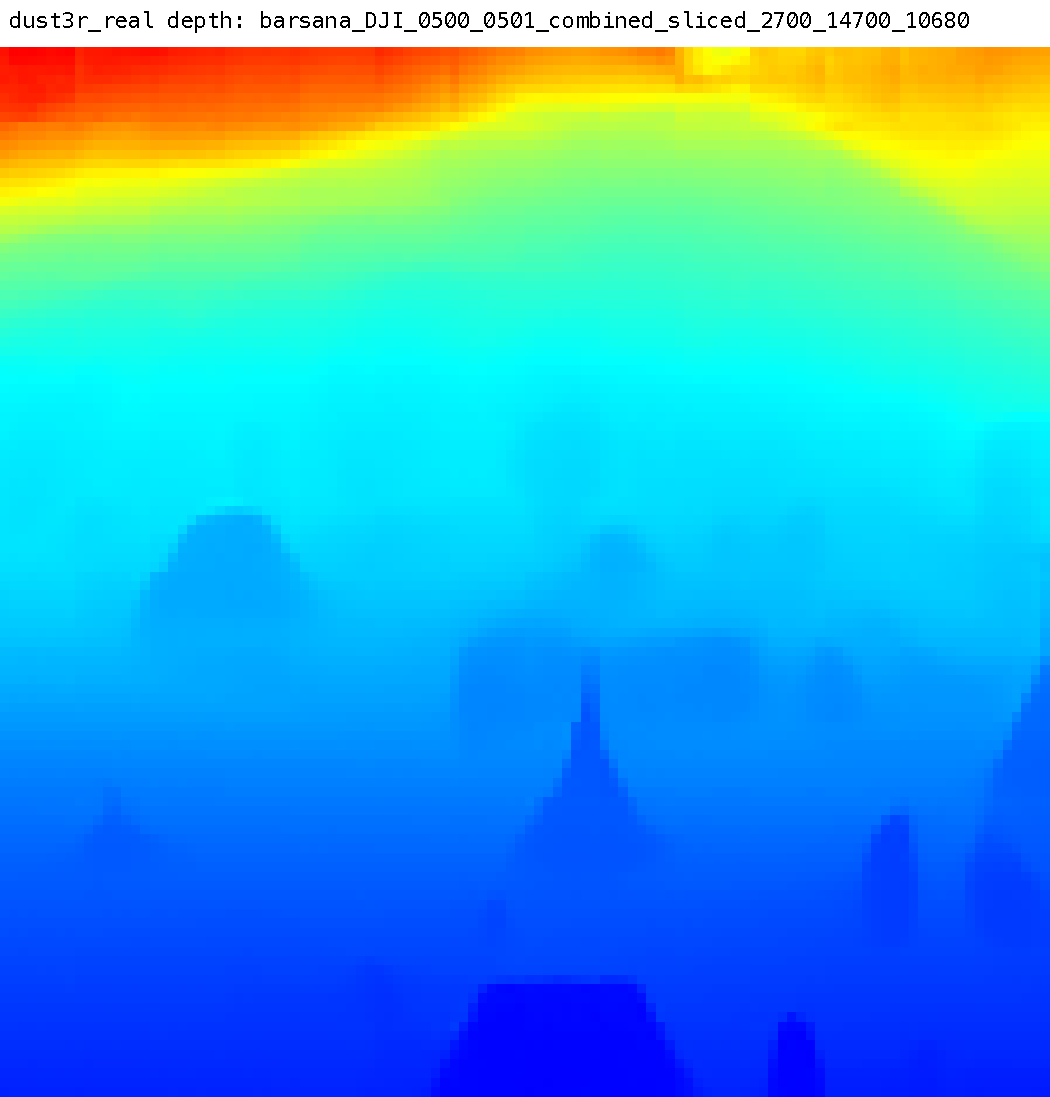
\includegraphics[width=\linewidth]{figures/dronescapes_dust3r_depth.pdf}

\small (a) Dronescapes, DUSt3R depth
\end{minipage}\hfill
\begin{minipage}[t]{0.31\linewidth}
\centering
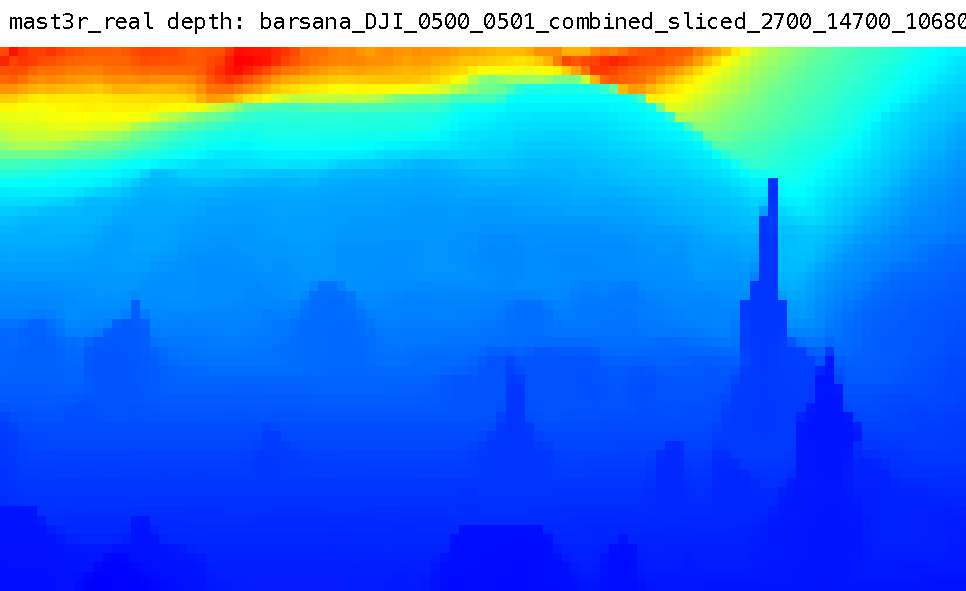
\includegraphics[width=\linewidth]{figures/dronescapes_mast3r_depth.pdf}

\small (b) Dronescapes, MASt3R depth
\end{minipage}\hfill
\begin{minipage}[t]{0.31\linewidth}
\centering
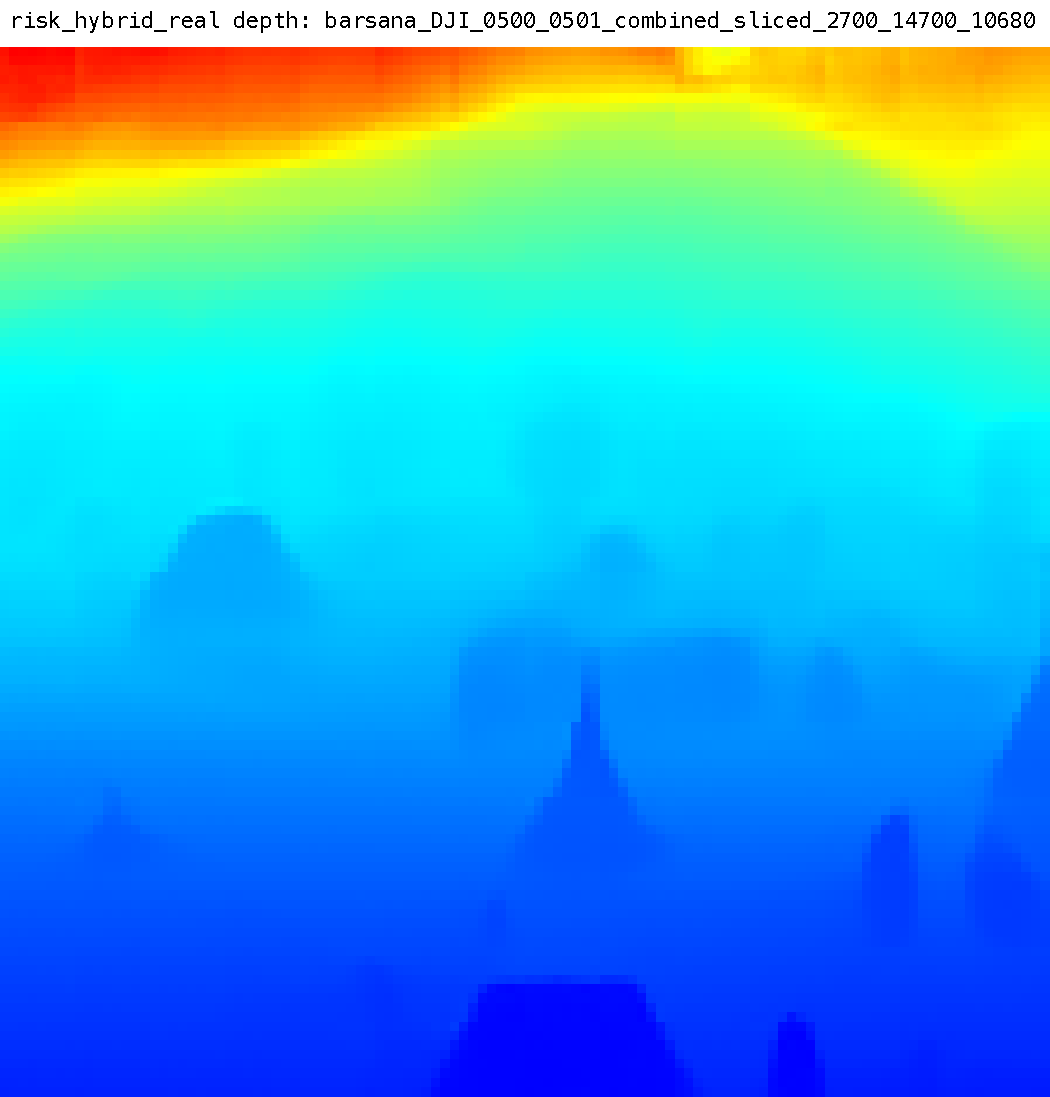
\includegraphics[width=\linewidth]{figures/dronescapes_risk_depth.pdf}

\small (c) Dronescapes, risk-hybrid depth
\end{minipage}

\vspace{0.8em}

\begin{minipage}[t]{0.31\linewidth}
\centering
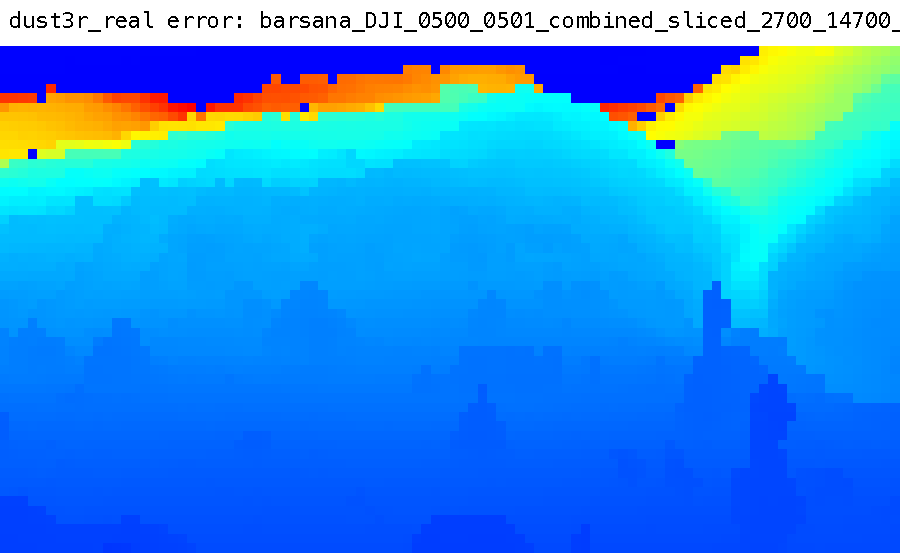
\includegraphics[width=\linewidth]{figures/dronescapes_dust3r_error.pdf}

\small (d) Dronescapes, DUSt3R error
\end{minipage}\hfill
\begin{minipage}[t]{0.31\linewidth}
\centering
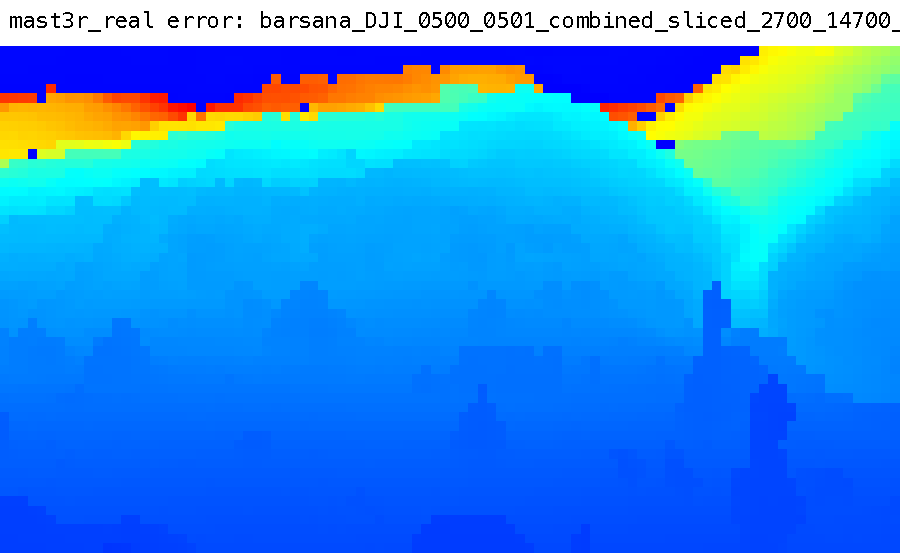
\includegraphics[width=\linewidth]{figures/dronescapes_mast3r_error.pdf}

\small (e) Dronescapes, MASt3R error
\end{minipage}\hfill
\begin{minipage}[t]{0.31\linewidth}
\centering
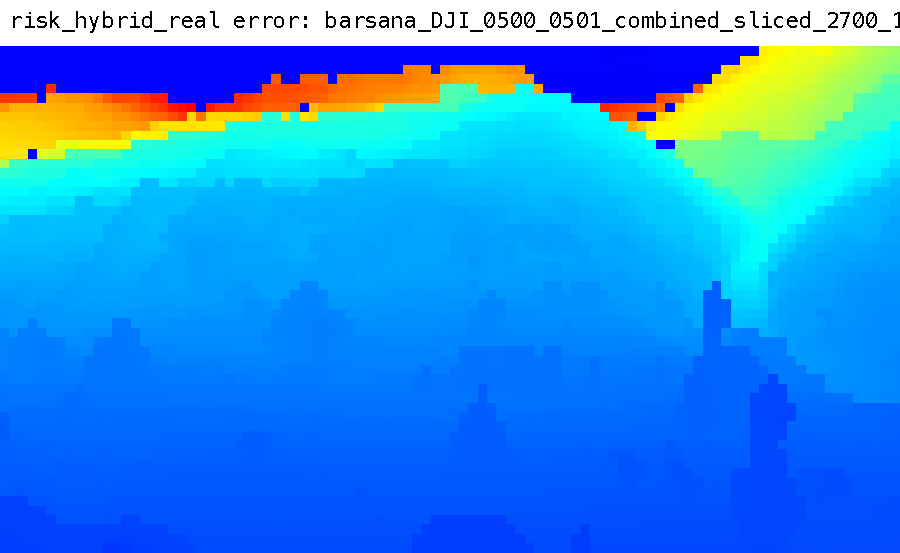
\includegraphics[width=\linewidth]{figures/dronescapes_risk_error.pdf}

\small (f) Dronescapes, risk-hybrid error
\end{minipage}

\vspace{0.8em}

\begin{minipage}[t]{0.31\linewidth}
\centering
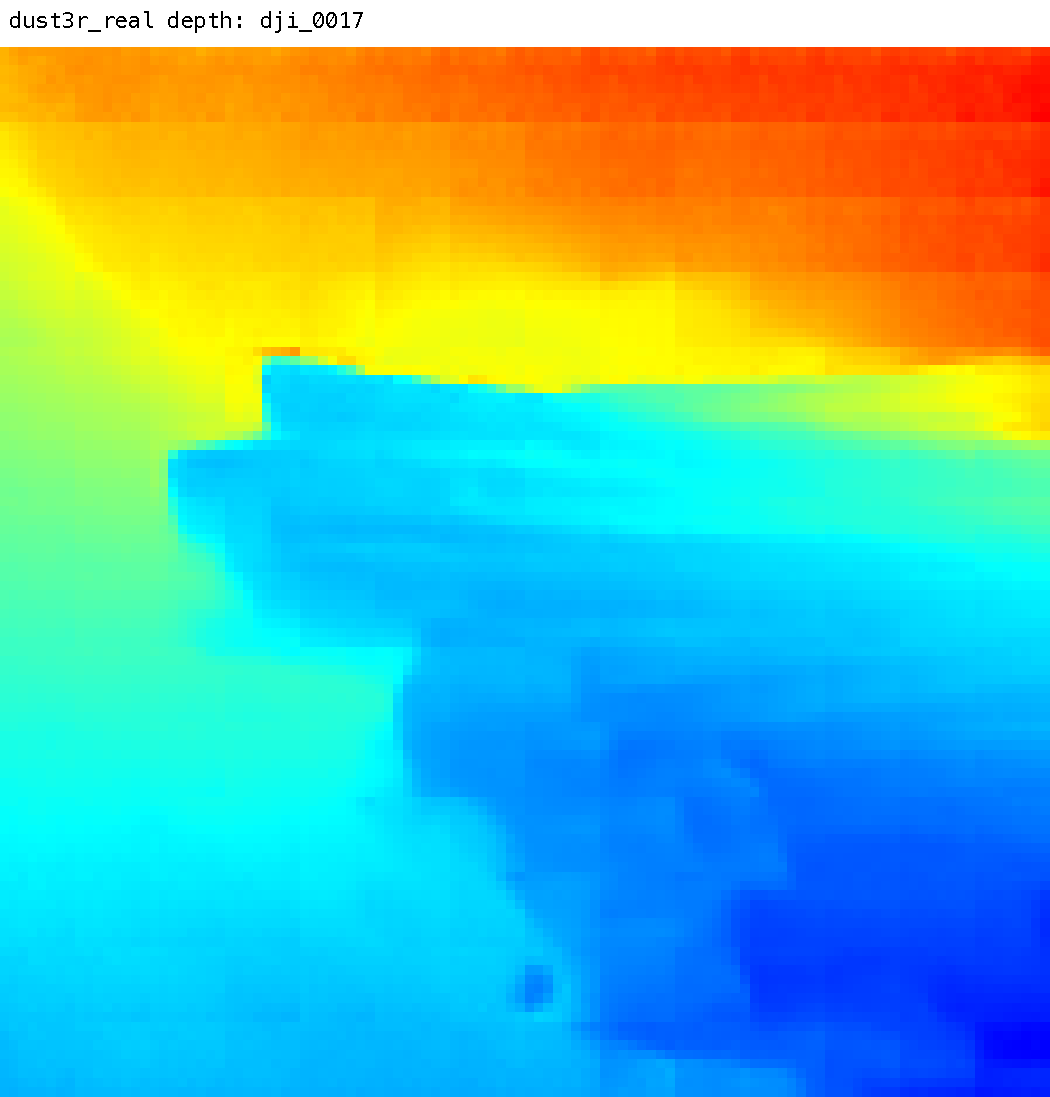
\includegraphics[width=\linewidth]{figures/odmdata_dust3r_depth.pdf}

\small (g) ODMData, DUSt3R depth
\end{minipage}\hfill
\begin{minipage}[t]{0.31\linewidth}
\centering
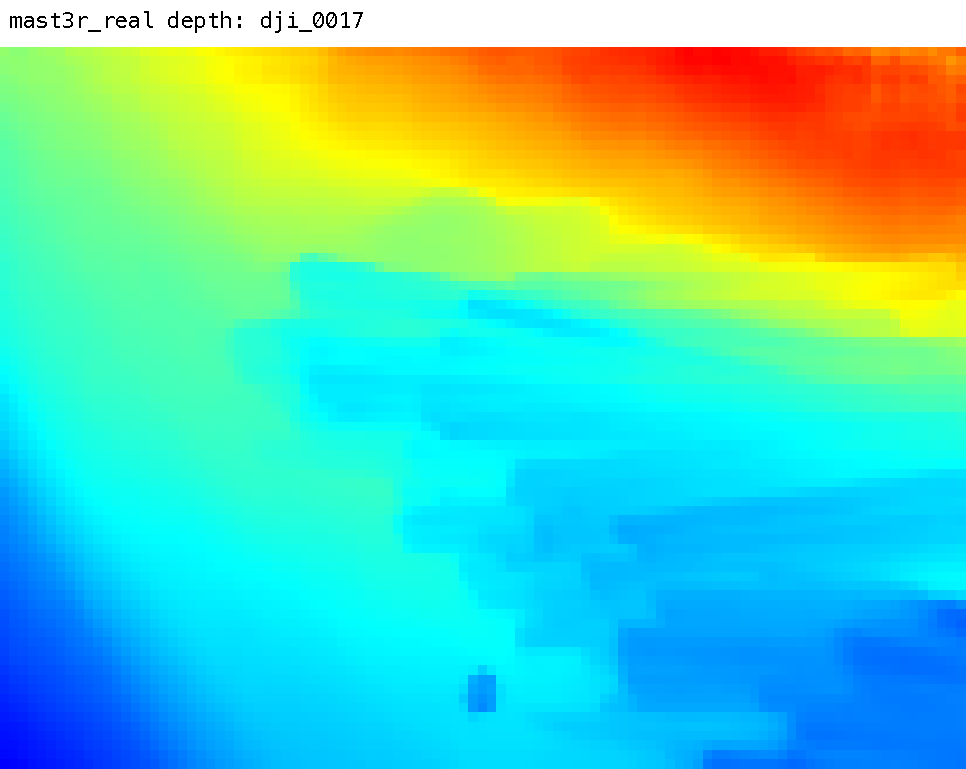
\includegraphics[width=\linewidth]{figures/odmdata_mast3r_depth.pdf}

\small (h) ODMData, MASt3R depth
\end{minipage}\hfill
\begin{minipage}[t]{0.31\linewidth}
\centering
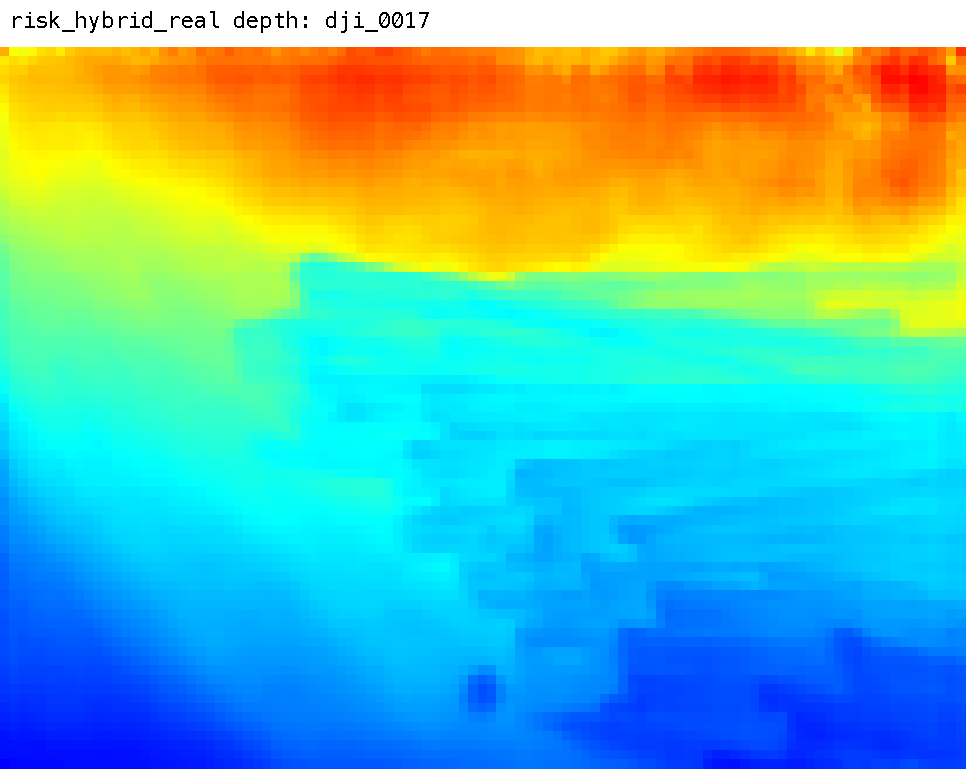
\includegraphics[width=\linewidth]{figures/odmdata_risk_depth.pdf}

\small (i) ODMData, risk-hybrid depth
\end{minipage}
\caption{Mega-figure 3x3 cho kết quả định tính. Risk-hybrid cải thiện rõ coarse behavior của DUSt3R và giữ được cấu trúc lớn của scene, nhưng vẫn chưa ổn định bằng MASt3R full-pass ở mọi vùng khó.}
\label{fig:qualitative-grid-thesis}
\end{figure}

\section{Thảo luận}

Từ các bảng và hình trên, có thể rút ra ba nhận xét chính.

Thứ nhất, \textbf{thế mạnh lớn nhất của risk-hybrid không phải là điểm số tuyệt đối tốt nhất, mà là hiệu quả phân bổ refinement budget}. Phương pháp này cho kết quả tốt hơn DUSt3R trên Dronescapes và giữ mức cạnh tranh trên ODMData trong khi chỉ refine một phần nhỏ số frame.

Thứ hai, \textbf{MASt3R vẫn là upper baseline mạnh hơn về độ chính xác}. Vì thế, nếu mục tiêu duy nhất là best accuracy, thì pipeline đề xuất hiện chưa đủ mạnh để thay thế full-pass MASt3R.

Thứ ba, \textbf{risk score hiện tại còn heuristic}. Nó đã đủ tốt để tạo ra tín hiệu nghiên cứu, nhưng chưa đủ giàu để học được những mẫu bất định phức tạp hơn. Đây là điểm cần mở rộng nếu muốn đề tài tiến xa hơn thành một hướng nghiên cứu mạnh.

\section{Giới hạn của đồ án}

Đồ án hiện còn ba giới hạn chính:
\begin{enumerate}[leftmargin=1.5em]
  \item risk score chưa được học từ dữ liệu mà vẫn dựa trên quy tắc thủ công;
  \item bộ thực nghiệm full với mọi suite lớn vẫn phụ thuộc mạnh vào điều kiện phần cứng;
  \item benchmark trên ODMData mới mang tính so sánh tương đối, chưa thay thế được một benchmark có ground-truth hình học trực tiếp.
\end{enumerate}

\chapter{Kết luận và hướng phát triển}

\section{Kết luận}

Đồ án đã hoàn thành ba việc cốt lõi. Thứ nhất, hệ thống hóa bối cảnh nghiên cứu của bài toán tái tạo 3D và xác định vị trí của UAV image-based reconstruction trong bức tranh chung. Thứ hai, đề xuất và hiện thực hóa một pipeline \textit{risk-guided hybrid refinement} dựa trên DUSt3R, MASt3R và chiến lược chọn frame theo rủi ro. Thứ ba, xây dựng được một repo benchmark độc lập và chạy thực nghiệm trên hai dataset thật.

Kết quả cho thấy selective refinement theo mức rủi ro là một hướng có cơ sở. Trong trạng thái hiện tại, phương pháp đề xuất chưa vượt MASt3R full-pass về độ chính xác tuyệt đối, nhưng đã thể hiện một câu chuyện rõ ràng hơn về \textbf{trade-off giữa chất lượng và chi phí tính toán}. Đây là kết luận hợp lý và trung thực nhất của đồ án.

\section{Hướng phát triển}

Các hướng mở rộng tiếp theo gồm:
\begin{enumerate}[leftmargin=1.5em]
  \item học trực tiếp risk score thay vì dùng heuristic tuyến tính;
  \item thử nghiệm chiến lược budget allocation động theo scene complexity;
  \item thêm các ablation như random selection, overlap-only, texture-only;
  \item tích hợp chặt hơn coarse prediction và refine prediction thay vì overwrite hoặc merge đơn giản;
  \item mở rộng sang các nhánh thời gian thực hoặc SLAM-aware reconstruction.
\end{enumerate}

\appendix
\chapter{Phụ lục: Hướng dẫn chạy nhanh}

Repo dự án: \url{https://github.com/duy12i1i7/GEO}

Lệnh tổng quát:
\begin{verbatim}
./run_geo_project.sh
\end{verbatim}

Chạy POC cân bằng trên Ubuntu + NVIDIA:
\begin{verbatim}
./scripts/run_poc_balanced_ubuntu_nvidia.sh
\end{verbatim}

Chạy full thermal-safe:
\begin{verbatim}
./scripts/run_full_thermal_safe_ubuntu_nvidia.sh
\end{verbatim}

\bibliographystyle{plainnat}
\bibliography{references}

\end{document}
